% !TeX spellcheck = de_DE
\documentclass{uebung_cs}
\usepackage{algo123}
\uebung{13}{}{}
\blattname{Dynamische Programmierung (Woche 13)}

\begin{document}
\textbf{Eigenständige Vorbereitung}
Lies \emoji{book} E Kapitel 3 ohne 3.6 und 3.9 und schau dir das \emoji{television} Video der Woche an.

\textbf{Zeichenlegende:}
\legende{}

%  \schriftlich
%  \bestehen
%  \mittel
%  \note
%  \spass

\begin{aufgabe}[Editieren]\mbox{}
    \begin{enumerate}
        \item\bestehen Welche Editiersequenz ist hier visualisiert und wie viele Editieroperationen wurden benutzt?
\begin{verbatim}
    P   L U   T   O
    P L A   N E T
\end{verbatim}
        \item\bestehen Fülle alle 25 Einträge der Tabelle \texttt{Edit[i,j]} mit $A=\texttt{PLUTO}$ und $B=\texttt{PLANET}$ aus. Gib die optimale Editiersequenz an.
        \item\mittel Die Tabelle \texttt{Edit[i,j]} hat $mn$ Einträge und braucht daher $O(mn)$ Platz. Wie kann das dynamische Programm für die Editiersequenz \emph{platzsparend} gemacht werden, sodass zu jedem Zeitpunkt nur noch ${O(\min\{m,n\})}$ Platz gebraucht wird? Die Laufzeit soll dabei asymptotisch gleich bleiben.
    \end{enumerate}
\end{aufgabe}

\paragraph{Hinweise zur Abgabe und zum Vorgehen bei Aufgaben des Typs \enquote{Dynamische Programmierung}.}
Im Buch [\href{https://jeffe.cs.illinois.edu/teaching/algorithms/book/Algorithms-JeffE.pdf}{Erickson}, Abschnitt 3.4] ist in kleinen Schritten beschrieben, wie man bei dynamischer Programmierung vorgeht.
Folge diesen Schritten!
Fang gar nicht erst an, über for-Schleifen nachzudenken, bevor du eine vollständige rekursive Lösung hast! Das beinhaltet eine klar verständliche deutsche oder englische Spezifikation der rekursiven Teilprobleme, die du löst.
In der Algorithmenentwicklung, in der Programmierung, und in den meisten Aufgaben des Lebens gilt immer: \textbf{Mach es zuerst korrekt, dann effizient.}

\begin{aufgabe}[Pascalsches Dreieck \schriftlich]\mbox{}\\
    Für die Binomialkoeffizienten gilt folgende Rekursionsformel:
    \begin{align*}
        \binom{n}{0}&=\binom{n}{n}=1&\quad\text{für alle $n\ge 0$, und}\\
        \binom{n}{k}&=\binom{n-1}{k-1}+\binom{n-1}{k}&\quad\text{für alle $n,k$ mit $ 1\le k \le n-1$.}
    \end{align*}
    Wir möchten eine Funktion implementieren, die $\binom{n}{k}$ ausrechnet.
    \begin{enumerate}
        \item\bestehen Entwirf zunächst eine rekursive Funktion \Call{RecBinom}{$n,k$}, die schlicht die Rekursionsformel rekursiv benutzt. Wie viele rekursive Aufrufe braucht \Call{RecBinom}{$n,k$}? Gib die Antwort in asymptotischer Notation in Abhängigkeit von $n$ und $k$ an.
        \item\bestehen Entwirf nun mit Hilfe von dynamischer Programmierung eine iterative Funktion \Call{IterBinom}{$n,k$}, die $O(nk)$ arithemtische Operationen ausführt und dabei $O(nk)$ Zahlen im Speicher hält.
        \item\mittel Entwirf nun mit Hilfe von platzsparender dynamischer Programmierung eine iterative Funktion \Call{IterBinom2}{$n,k$}, die ebenfalls $O(nk)$ arithmetische Operationen braucht, dabei aber nur $O(k)$ Zahlen im Speicher halten muss.
    \end{enumerate}
\end{aufgabe}
\begin{aufgabe}[Betriebsfeier \mittel]
    Du organisierst die jährliche Betriebsfeier bei der Algorithmen-Bank.
    Die Mitarbeiter:innen der Bank sind in einer strikten Hierarchie angeordnet: ein Baum, in dem die Eigentümerin der Bank die Wurzel darstellt.
    Die allwissende Personalabteilung hat für jede:n Angestellte:n eine reelle Zahl berechnet, die angibt, wie \enquote{lustig} diese Person ist.
    Damit die Feier entspannt bleibt, gibt es folgende Einschränkung für die Gästeliste:
    ein:e Mitarbeiter:in darf nicht an der Feier teilnehmen, wenn seine:ihre direkte Vorgesetze teilnimmt.
    Andererseits \emph{muss} die Eigentümerin an der Feier teilnehmen, obwohl sie nicht besonders lustig ist; es ist ja schließlich auch ihre Firma.
    Beschreibe und analysiere einen Algorithmus, der diejenige Gästeliste für die Betriebsfeier berechnet, die die Summe aller \enquote{lustig} Bewertungen der Gäste maximiert.
\end{aufgabe}

\begin{aufgabe}[Genaues Rückgeld]
    In einem früheren Leben hast du als Kassierer:in in der verlorenen antarktischen Kolonie Nadiria gearbeitet, wo du die meiste Zeit des Tages Rückgeld an deine Kund:innen gegeben hast.
    Weil Papier ein knappes und wertvolles Gut in der Antarktis ist, gab es das Gesetz, dass Kassierer:innen immer die kleinstmögliche Anzahl an Geldscheinen zurückgeben müssen.
    Die Währung von Nadiria heißt Traumdollar und war in den folgenden Scheinen verfügbar:
    \$1,
    \$4,
    \$7,
    \$13,
    \$28,
    \$52,
    \$91,
    \$365.
    \begin{enumerate}
        \item\bestehen Der gierige Wechselalgorithmus nimmt immer den größten Schein, der kleiner ist als das noch zu gebende Rückgeld. Zum Beispiel, um \$122 mit dem gierigen Algorithmus zurückzugeben, nehmen wir zuerst einen \$91 Schein, dann einen \$28 Schein, und am Ende drei \$1 Scheine. Gib ein Beispiel an, in dem der gierige Algorithmus mehr Traumdollarscheine als Wechselgeld gibt als die minimal mögliche Anzahl. \emph{Hinweis: Es könnte einfacher sein, ein kleines Programm zu schreiben, als von Hand ein Beispiel zu konstruieren.}
        \item\mittel Beschreibe und analysiere einen rekursiven Algorithmus, der für eine gegebene Zahl $k$ die kleinste Anzahl an Scheinen berechnet, die benötigt werden, um $k$ Traumdollar Rückgeld zu geben. (Mach dir erstmal keine Gedanken darüber, wie man den Algorithmus schnell macht; stell einfach sicher, dass er korrekt ist.)
        \item\mittel Beschreibe einen Algorithmus, der mithilfe von dynamischer Programmierung dasselbe algorithmische Problem löst. (Dieser Algorithmus soll schnell sein.)
    \end{enumerate}
\end{aufgabe}

\begin{aufgabe}[Maximales Teilfeld II \mittel]
    Erinnere dich zurück an die Aufgabe zu den maximalen Teilfeldern (Aufgabe 6 in Woche 3).
    Eine Lösung nutzt eine rekursive Funktion
    \Call{MaxTeilfeld}{$j$}, die die Summe eines maximalen Teilfelds ausrechnet, das in $j$ endet. Das heißt, die Funktion liefert unter den Teilfeldern $A[0..j]$, $A[1..j]$, $\dots$, $A[j..j]$ die maximale Summe.
    Ohne auf deine Notizen zu schauen, stelle zunächst einen einfachen rekursiven Algorithmus für diese Funktion auf. Wende dann dynamische Programmierung an, um den Algorithmus effizient zu machen. Hier ist noch einmal der Text aus der Aufgabenstellung:

    Sei $A \in \mathbb{Z}^n$ als ein Feld $A[0, \dots, n-1]$ gespeichert.
	Ein Teilfeld von $A$ ist ein genau dann ein \textit{maximales Teilfeld} $A[i..j]$ mit $0\leq i\leq j\leq n-1$, wenn die Summe $A[i] + A[i+1] + \cdots + A[j]$ maximal über alle möglichen Teilfelder ist.
    Beschreibe und analysiere einen Algorithmus, der mithilfe von dynamischer Programmierung die Summe eines maximalen Teilfelds von $A$ in Zeit $O(n)$ berechnet.
\end{aufgabe}

% \begin{aufgabe}[Palindromische Wege II]
%     Erinnere dich zurück an die Aufgabe zu den palindromischen Wegen (\emoji{star} in Woche 6).
%     Eine Lösung benutzt eine rekursive Funktion \Call{HasPalindromicWalk}{$u,v,i$}, die feststellt, ob es einen palindromischen Weg von $u$ nach $v$ der Länge $i$ gibt.
%     Ohne auf deine Notizen zu schauen, stelle den rekursiven Algorithmus für diese Funktion erneut auf. Wende dann dynamische Programmierung an, um den Algorithmus effizient zu machen. Hier ist noch einmal der Text aus der Aufgabenstellung:

%     Ein \emph{Palindrom} über dem Alphabet $\{\texttt{R},\texttt{B}\}$ ist eine Zeichenkette $s_1,s_2,s_3,\dots,s_n\in\{\texttt{R},\texttt{B}\}$, sodass $s_i=s_{n-i+1}$ für alle $i\in\{1,\dots,n\}$. Zum Beispiel sind \texttt{BRBRB} und \texttt{RBBR} Palindrome, aber \texttt{RBB} und \texttt{BRRR} nicht.

% Sei $G$ ein beliebiger gerichteter Graph, in dem jede Kante entweder rot oder blau gefärbt ist, und seien $s,t$ zwei Knoten.
% Beschreibe einen Algorithmus, der entweder einen Weg von $s$ nach $t$ berechnet, für den die Sequenz von rot und blau entlang der Kanten des Weges ein Palindrom ist, oder korrekterweise feststellt, dass kein solcher Weg existiert.

% \emph{Zur Erinnerung:} Ein Weg von $s$ nach $t$ darf sich selbst überlappen, das heißt, ein Weg muss nicht unbedingt einfach sein.
% \end{aufgabe}

\begin{aufgabe}[RNA]
    \emph{Ribonucleic acid} (RNA) ist eine lange Kette von Millionen Nukleotiden von vier verschiedenen Typen:
    Adenin (\verb|A|), Cytosin (\verb|C|), Guanin (\verb|G|), und Uracil (\verb|U|). Die \emph{Sequenz} eines RNA-Moleküls ist eine Zeichenkette $b[1\dots n]$, wobei jedes Zeichen $b[u]\in\{\texttt{A}, \texttt{C}, \texttt{G}, \texttt{U}\}$ zu einem Nukleotid korrespondiert.
        Manchmal mutiert ein Virus und die RNA-Sequenz verändert sich leicht. Deine Aufgabe ist es nun, für zwei gegebene RNA-Sequenzen herauszufinden, wie ähnlich diese sich sind; damit kann man Rückschlüsse ziehen darauf, wie ähnlich sich zwei Virusvarianten sind. Aber nicht jede Änderung in der RNA ist gleich wahrscheinlich! Wir haben nun folgende (fiktive) Ähnlichkeitsmatrix $M[a,b]$ gegeben, die für jede Punktmutation (=Substitution) angibt, wie wahrscheinlich diese ist:

        \begin{tabular}{ccccc}
                      & \texttt{A}  & \texttt{G}  & \texttt{C} & \texttt{U}\\
           \texttt{A} & $10$ & $-1$ & $-3$ & $-4$\\
           \texttt{G} & $-1$ & $ 7$ & $-5$ & $-3$\\
           \texttt{C} & $-3$ & $-5$ & $ 9$ & $ 0$\\
           \texttt{U} & $-4$ & $-3$ & $ 0$ & $ 8$\\
        \end{tabular}

        Je größer die Zahl ist, desto wahrscheinlicher soll die entsprechende Substitution sein.
        Zum Beispiel hat eine Substitution von C auf G einen Ähnlichkeitwert von -5, aber ein korrektes Alignment von G mit G hat einen Ähnlichkeitswert von 7.
        Außerdem definieren wir noch einen Wert $d=-5$, der den Ähnlichkeitswert einer Einfügen oder Löschen Operation auf $-5$ setzt.
        Der Ähnlichkeitswert einer Editiersequenz ist die Summe der Ähnlichkeitswerte für jede Spalte.
        \begin{enumerate}
            \item\bestehen Was ist der Ähnlichkeitswert dieser Editiersequenz?
\begin{verbatim}
    G A U  
    C   C G
\end{verbatim}
            \item\mittel Wie muss das dynamische Programm für die Edit Distance angepasst werden, um eine Editiersequenz zu berechnen, die einen möglichst großen Ähnlichkeitswert erzeugt?
        \end{enumerate}
\end{aufgabe}

\begin{aufgabe}[Sekundärstruktur]
    \textit{\footnotesize For an English version of this exercise, see [\href{https://jeffe.cs.illinois.edu/teaching/algorithms/book/Algorithms-JeffE.pdf}{Erickson}, page 149]}.
    \emph{Ribonucleic acid} (RNA) ist eine lange Kette von Millionen Nukleotiden oder \emph{Basen} von vier verschiedenen Typen:
    Adenin (\verb|A|), Cytosin (\verb|C|), Guanin (\verb|G|), und Uracil (\verb|U|). Die \emph{Sequenz} eines RNA-Moleküls ist eine Zeichenkette $b[1\dots n]$, wobei jedes Zeichen $b[i]\in\{\texttt{A}, \texttt{C}, \texttt{G}, \texttt{U}\}$ zu einer Basis korrespondiert.
    Zusätzlich zu den chemischen Verbindungen zwischen adjazenten Basen in der Sequenz können auch Wasserstoffbrückenbindungen zwischen manchen Basenpaaren entstehen.
    Die Menge der gebundenen Basenpaare heißt die \emph{Sekundärstruktur} des RNA-Moleküls.
    
    Wir sagen, dass zwei Basenpaare $(i,j)$ und $(i',j')$ mit $i<j$ und $i'<j'$ sich \textbf{\emph{überlappen}}, wenn $i<i'<j<j'$ oder $i'<i<j'<j$ gilt. In der Praxis überlappen sich die meisten Basenpaare nicht. Überlappende Basenpaaren bilden sogenannte Pseudoknoten in der Sekundärstruktur, die essenziell für bestimmte Funktionen der RNA sind, aber schwierig vorhergesagt werden können.
    
    Wir wollen jetzt die bestmögliche Sekundärstruktur für eine gegebene RNA-Sequenz berechnen. Wir nehmen das folgende vereinfachte Modell der Sekundärstruktur an:
    \begin{itemize}
        \item Jede Basis kann mit höchstens einer weiteren Basis eine Bindung eingehen.
        \item Nur \verb|A-U| Paare und \verb|C-G| Paare können gebunden sein.
        \item Paare der Form $(i,i+1)$ und $(i,i+2)$ können sich nicht binden.
        \item Gebundene Basenpaare können sich nicht überlappen.
    \end{itemize}
    Diese letzte (und am wenigsten realistische) Einschränkung erlaubt es uns, die Sekundärstruktur der RNA als eine Art fetten Baum zu visualisieren, siehe \cref{fig:RNA}.
    \begin{figure}[ht]
        \begin{center}
            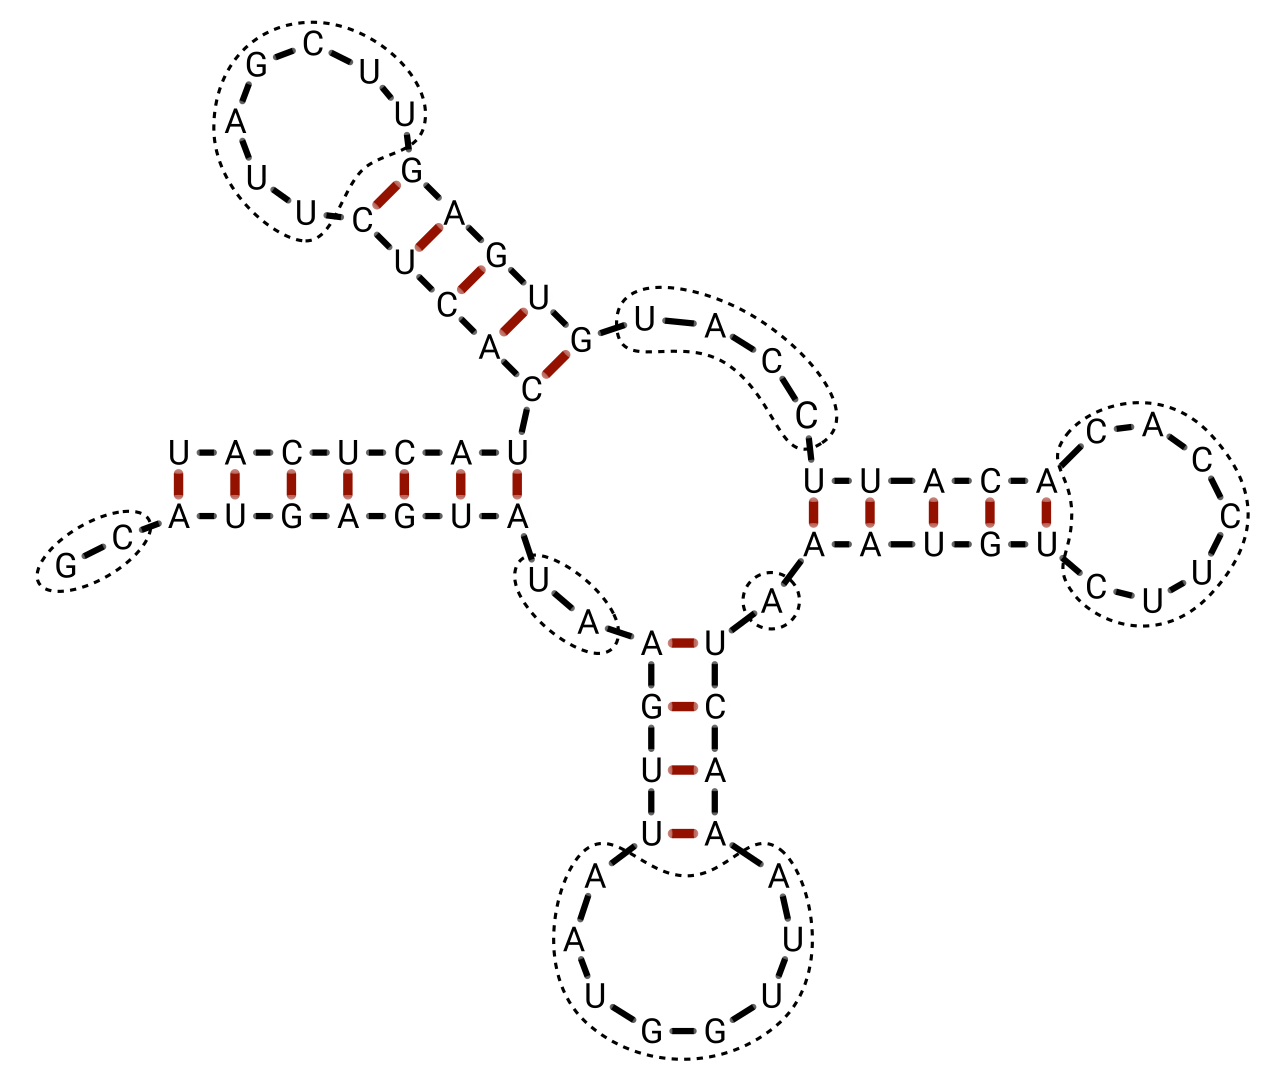
\includegraphics[width=.5\textwidth]{RNA-secondary-structure.png}
        \end{center}
    \caption{\label{fig:RNA}Beispiel einer RNA Sekundärstruktur mit 21 gebundenen Basenpaaren, die durch die fetten roten Linien gekennzeichnet sind. Lücken sind durch die gepunkteten Kurven gekennzeichnet. Diese Struktur hat eine Bewertung von $2^2+2^2+8^2+1^2+7^2+4^2+7^2=187$.}
    \end{figure}
    \begin{enumerate}
        \item\mittel Beschreibe und analysiere einen Algorithmus, der die größtmögliche \emph{Anzahl} an gebundenen Basenpaaren in der Sekundärstruktur einer gegebenen RNA-Sequenz berechnet.
        \item\note Eine \emph{Lücke} in der Sekundärstruktur ist ein maximaler Teilstring von ungebundenen Basen. Große Lücken sind chemisch instabil, daher sind Sekundärstrukturen mit kleineren Lücken viel wahrscheinlicher.
        Um diese Präferenz einzubeziehen, definieren wir jetzt die \emph{Bewertung} einer Sekundärstruktur als die Summe der \emph{Quadrate} der Längen aller Lücken; siehe die obige Abbildung. (Diese Bewertung ist fiktional; um die tatsächliche RNA-Struktur vorherzusagen braucht man \emph{deutlich} komplizierte Bewertungsmethoden.)
    
        Beschreibe und analysiere einen Algorithmus, der für eine gegebene RNA-Sequenz die kleinstmögliche Bewertung einer Sekundärstruktur berechnet.
    \end{enumerate}
\end{aufgabe}

\end{document}
